%=======================02-713 LaTeX template, following the 15-210 template==================
%
% You don't need to use LaTeX or this template, but you must turn your homework in as
% a typeset PDF somehow.
%
% How to use:
%    1. Update your information in section "A" below
%    2. Write your answers in section "B" below. Precede answers for all 
%       parts of a question with the command "\question{n}{desc}" where n is
%       the question number and "desc" is a short, one-line description of 
%       the problem. There is no need to restate the problem.
%    3. If a question has multiple parts, precede the answer to part x with the
%       command "\part{x}".
%    4. If a problem asks you to design an algorithm, use the commands
%       \algorithm, \correctness, \runtime to precede your discussion of the 
%       description of the algorithm, its correctness, and its running time, respectively.
%    5. You can include graphics by using the command \includegraphics{FILENAME}
%
\documentclass[11pt]{article}
\usepackage{amsmath,amssymb,amsthm}
\usepackage{amsbsy}
\usepackage{graphicx}
\usepackage[margin=1in]{geometry}
\usepackage{fancyhdr}
\setlength{\parindent}{0pt}
\setlength{\parskip}{5pt plus 1pt}
\setlength{\headheight}{13.6pt}
\newcommand\question[2]{\vspace{.25in}\hrule\textbf{#1: #2}\vspace{.5em}\hrule\vspace{.10in}}
\renewcommand\part[1]{\vspace{.10in}\textbf{(#1)}}
\newcommand\algorithm{\vspace{.10in}\textbf{Algorithm: }}
\newcommand\correctness{\vspace{.10in}\textbf{Correctness: }}
\newcommand\runtime{\vspace{.10in}\textbf{Running time: }}
\pagestyle{fancyplain}
\lhead{\textbf{\NAME\ (\ANDREWID)}}
% \chead{\textbf{MP\HWNUM}}
% \rhead{\today}
\begin{document}\raggedright
%Section A==============Change the values below to match your information==================
\newcommand\NAME{Renqin Cai}  % your name
\newcommand\ANDREWID{rc7ne}     % your andrew id
% \newcommand\HWNUM{3}              % the homework number
%Section B==============Put your answers to the questions below here=======================

% no need to restate the problem --- the graders know which problem is which,
% but replacing "The First Problem" with a short phrase will help you remember
% which problem this is when you read over your homeworks to study.



% \question{1}{The First Problem} 

% \part{a} \algorithm Describe algorithm here

% \correctness This is an argument  that this algorithm returns the correct answer.

% \runtime Describe here, in big-Oh, the running time and your reasoning for it.

% \part{b}

% \question{2}{The second problem}
% \begin{align*}
% \lambda_u(t) = \lambda_u(0)+\sum_{t_j<t} S_{t_j} I_{jk} S_{t}
% \end{align*}
% where $\lambda_u(t)$ is the intensity function. $\lambda_u(0)$ is the basic intensity, representing the probablity that the user $u$ browse a random item spontaneously. $\sum_{t_j<t}$ is to capture the influence from previous events on the current browsing behavior happening at time $t$. The $S_{t_j}$ is the state of one previous event happening at time $t_j$. The $S_{t}$ is the state of the current browsing event. $I$ is the influence matrix, whose row and column represent the items. The element $I_{jk}$ is the influence from item $i_j$ browsed at $t_j$ on the item $i_k$ browsed at $t$. 

% After selecting the timestamp of the event, the generative process of the item is:

The figure \ref{fig:browsingsequence} visualizes the generation of the browsing sequence. 

\begin{figure}[h]
\centering
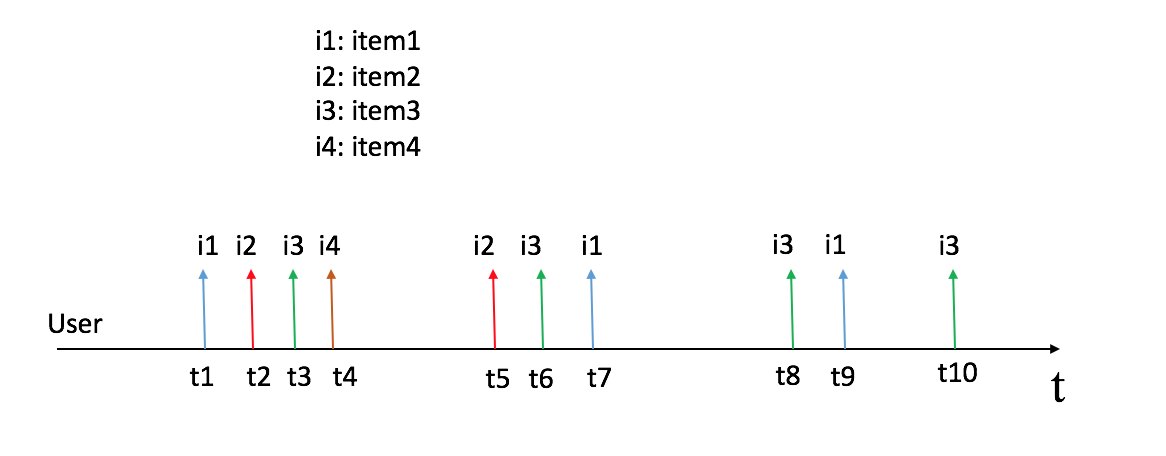
\includegraphics[width=0.9\textwidth]{browsingSequence.png}
\caption{browsing sequence of a purchase of a user}
\label{fig:browsingsequence}
\end{figure}

% We use a latent vector $u$ to represent a user and a latent vector $i$ to represent an item. The vector $u(t)$ means the user's preferences (aspect weights) at time $t$. On the other hand, the vector $i(t)$ means the item $i's$ attributes (aspect qualities), which is browsed at time $t$. We believe the attributes of browsed items can shape the user's preferences over time and a user's browsing history can be separated into several stages. In different stages, the influence of item's attributes on the user's preferences could be different, indicating different accepting patterns of items' attributes. To capture this dynamic patterns, we use $s_{t}$ to represent the user $u's$ accepting pattern at time $t$ and $\alpha_u^{s_t}$ to represent the value of accepting rate.  Thus, at time $t$, the preference of a user $u$ can be represented as, 

% In order to differentiate the purchasing behaviors and browsing behaviors, we use $u_s$ to represent the user $u$'s shopping preference vector and $u_b$ to represent the user $u$'s browsing preference vector. The vector $u_s(t)$ means the user's shopping preference (aspect weights) at time $t$. On the other hand, the vector $u_b(t)$ represents the user's browsing preference at time $t$. And they are linked via 
% \begin{align*}
%     u_s(t) = u_b(t) + \epsilon
% \end{align*}
% where $\epsilon \sim Gaussian(\mu, \sigma)$ represents the deviation of shopping preference to browsing preference.

We use $u_i$ to represent the user's browsing preference vector and $v$ to represent the item's attribute vector. $V$ represents the whole set of items.  

We believe attributes of browsed items can shape both user's browsing preferences and user's purchasing preferences over time. $\alpha$ represents the shaping pattern adopted by user $u$. Shaping patterns $\{\alpha_1, ..., \alpha_m, ..., \alpha_M\}$ are shared among users. Thus, the browsing preference of the user $u$ at time $t$ can be represented as, 

\begin{align}
\label{user_preference_vec}
\vec{u}_i(t) = \vec{u}_i(0)+\sum_{t_j<t} (\vec{\alpha}_{t_j}\odot\vec{v}_{t_j}) Kernel(t,t_j)
\end{align}
where the $Kernel(t, t_j)$ is a time decaying function, maybe exponential function, and $\odot$ means the element-wise product of two vectors. ${\vec{\alpha}}_{t_j}\odot\vec{v}_{t_j}$ captures how the browsed items change the user's preference dimension-wise. Browsing an item may affect a proportion of dimensions of users' preferences.  

In addition, we believe that not all browsed items will influence the users' preferences, so we use a latent variable $z$ to distinguish whether the browsed item affects the user's preference. When $z=1$, the browsed item affects the user's preference. When $z=0$, the browsed item does not affect the user's preference. So the Eq.\ref{user_preference_vec} transforms into the following format,
\begin{align}
\label{user_preference_vec_z}
\vec{u}_i(t) = (1-z_t)\vec{u}_i(t-1)+z_t\big\{ \vec{u}_i(0)+\sum_{t_j<t} (\vec{\alpha}_{t_j}\odot\vec{v}_{t_j}) exp\big(-\gamma_1 (t-t_j)\big)\big\}
\end{align}
where the $Kernel(t,t_j)$ is replaced with $exp\big(-\gamma_1 (t-t_j)\big)$

Since latent variable $z$ is a binary variable, we assume it is generated through a Bernoulli distribution. In addition, we impose Beta distribution as a prior to this Bernoulli distribution.

The generation of $t$ is modeled via a Hawkes Process:
\begin{align}
\lambda(t) = \lambda_0+\sum_{t_j<t} z_{t_j}\langle\vec{\beta}_{u_i,t_j}^1\,,\vec{v}_{t_j}\rangle\exp\big(-\gamma_2 (t-t_j)\big) +\sum_{t_j<t} (1-z_{t_j})\langle\vec{\beta}_{u_i, t_j}^0\,,\vec{v}_{t_j}\rangle \exp\big(-\gamma_2 (t-t_j)\big)
\end{align}

% We believe that the influence of items on the users' preferences and the influence of items on the users' clicking rate should be captured by different parameters. So we use Hawkes Process to capture the rate of generating a click as the following equation shows.

% \begin{align}
% \lambda^*_{u_i}(t) = \lambda^*_{u_i}(t_0)+\sum_{t_j<t} (\vec{\beta}_{u_i,t_j})^T\vec{v}_{t_j}Kernel(t, t_j)
% \end{align}


% $\sum_{t_j<t}$ captures the sequential influence of previous browsing items on the current browsing behavior. $u_b(0)$ represents the user's intrinsic browsing preference. $\alpha_{t_j}$ is the shaping pattern at time $t_j$, which could be one value of $\{\alpha_1, ..., \alpha_m, ..., \alpha_M\}$. The intensity of adopting the shaping pattern $\alpha_{m}$ is 
% \begin{align*}
%     \lambda_{\alpha_m}(t) = \lambda_{\alpha_m}(0)+\sum_{t_j<t}A_{\alpha_{t_j}\alpha_{m}} Kernel(t,t_j)
% \end{align*}

% We use a latent vector $u$ to represent a user and a latent vector $x$ to represent an item. The vector $u(t)$ means the user's preferences (aspect weights) at time $t$. On the other hand, the vector $x_t$ means the item $x$'s attributes (aspect qualities), which is browsed by the user at time $t$. We believe the attributes of browsed items can shape the user's preferences over time and how the attributes of browsed items shape the user’s preferences can be categorized into groups shared by users. We use $\alpha_{t}$ to represent the shaping pattern at time t. Thus, at time $t$, the preference of a user $u$ can be represented as,

% \begin{align}
% u(t) = u_0+ \sum_{t_j<t} \alpha^{t_j}x_{t_j}
% \end{align}

% $\sum_{t_j<t}$ captures the sequential influence of previous browsing items on the current browsing behavior. And for time $t_j$, the corresponding shaping pattern is $\alpha^{t_j} \sim Gaussian (\mu, \sigma)$.
% \begin{align*}
% u(t) = u_0+ \sum_{t_j<t} \alpha_u^{s_{t_j}}i(t_j) 
% \end{align*}
Given the current user's browsing preferences $u_i(t)$ and items' attributes, the probability of browsing the item $v$ at time $t$ is
\begin{align}\label{itemProbability}
p(v_t) = \frac{exp(\vec{u}_i(t)^T\vec{v}_t)}{\sum^V_v exp(\vec{u}_i(t)^T\vec{v})}
\end{align}
where $v_t$ means the item attributes vector browsed at time $t$. 

The whole generative process of the sequence data is: \\
for each sequence of a user 
\begin{enumerate} \denselist
\item sample $\theta\sim Beta(a, b)$
\item for each action in the sequence
    \begin{enumerate}\denselist
    \item sample the on/off variable $z \sim \theta$
    \item sample the timestamp $t \sim \lambda(t)$
    \item draw the user preference vector $\vec{u}_i(t)$ according to  Eq.\ref{user_preference_vec_z}
    \item browse the item $v$ with probability $p(v_t)$ according to Eq.\ref{itemProbability}
    \end{enumerate}
\end{enumerate}
% Moreover, the intensity of shopping the item $x$ is 
% \begin{align*}
%     \lambda_s(t) = u_s(t)^Tx
% \end{align*}

If we think of whether browsing an item or not at each timestamp as a binary classification problem, our setting is that we use one set of parameters of logistic regression to predict each browsing behavior and the parameters are linked via the Hawkes Process as the equation 1 shows. Our current setting of logistic regression, which we call “Hawkes Process Logistic Regression”, lies between two extreme settings of logistic regression. One extreme is using one set of parameters of logistic regression to predict the browsing behaviors of the whole sequence. The other extreme is for each browsing behavior using one set of parameters of logistic regression to predict. To verify whether our intermediate setting can improve the accuracy, we can first verify another simpler intermediate setting that we divide a sequence into multiple groups of browsing behaviors and for each group we use a logistic regression to predict, which we call “Group Logistic Regression”. If “Group Logistic Regression” can work better than two extremes, we may expect our current setting can perform best among these models. Since how to divide the group matters a lot in “Group Logistic Regression” and it is difficult to achieve an ideal division, “Hawkes Process Logistic Regression” which do not need to divide the sequence into groups may outperform “Group Logistic Regression”. As a result, “Hawkes Process Logistic Regression” may outperform other models.


% $\sum_{t_j<t}$ captures the sequential influence from previous events happening at $\{t_j<t\}$ on the current browsing behavior. And for time $t_j$, the corresponding accepting pattern is $s_{t_j}$, whose accepting rate is $\alpha_u^{s_{t_j}}\sim Gaussian(\mu, \sigma)$. 

% Given the current user's preferences $u(t)$ and items' attributes, the probability of browsing the item $k$ at time $t$ is 
% \begin{align*}
% p(k) = \frac{exp(u(t)^Tk)}{\sum_{i} exp(u(t)^Ti)}
% \end{align*}
% where $i$ is the item $i's$ latent vector of the item set.

% One extension of the current model is:
% 1. The accepting pattern are shared across users. we can add a $HDP$ to model the phenomena that a sequence is composed of multiple patterns which shared across sequences.


% Some problems are left to address:
% 1. How to evaluate the assumption that a sequence can be separated into multiple stages is valid through some experiments on $\alpha$?
% 2. Whether we need to assume the item's attributes are dynamic? Currently, we treat latent vector of an item $i$ is static
% 3. Whether the accepting rate should be modeled as a matrix? Currently, we treat it as a scalar, which means the accepting rate for every aspect is the same. Or should we treat $\alpha$ as a vector and change $\alpha_u^{s_{t_j}}i(t_j)$ into element-wise multiplication $\alpha_u^{s_{t_j}} \times i(t_j)$?
% We assume a user's browsing history can be separated into several stages, which indicate different browsing patterns. In different states, the influence of a browsed item on a user can be different. At the early stage of this purchase, since a user browse many items, the influence from an individual item can be rather small. At the final stage of this purchase, the current browsed item is presumably to have a strong influence on the choice of the item to browse next. The stages are represented as $S$.

% \begin{align*}
% \lambda_u(t) = \lambda_u(0)+\sum_{t_j<t} S_{t_j} U_{uj} S_{t}
% \end{align*}
% where $\lambda_u(t)$ is the intensity function. $\lambda_u(0)$ is the basic intensity, representing the probability that the user $u$ browse a random item spontaneously. $\sum_{t_j<t}$ is to capture the influence from previous events on the current browsing behavior happening at time $t$. The $S_{t_j}$ is the stage of one previous event happening at time $t_j$. The $S_t$ is the stage of the current browsing event. $U$ is the influence matrix, whose rows represent users and columns represent items. The element $U_{uj}$ means the influence of historical browsing event happening at $t_j$ on the user $u$. 

% % where $\lambda_u(t)$ is the intensity function. $\lambda_u(0)$ is the basic intensity, representing the probablity that the user $u$ browse a random item spontaneously. $\sum_{t_j<t}$ is to capture the influence from previous events on the current browsing behavior happening at time $t$. The $S_{t_j}$ is the state of one previous event happening at time $t_j$. The $S_{t}$ is the state of the current browsing event. $I$ is the influence matrix, whose row and column represent the items. The element $I_{jk}$ is the influence from item $i_j$ browsed at $t_j$ on the item $i_k$ browsed at $t$. 

% We assume an item can be represented by a $K$ dimensional vector of attributes $(a_1, ..., a_K)$. After selecting the timestamp of the event happening at time $t$, the generative process of the item is:
% \begin{align*}
% a_k \sim Gaussian(a^{parent(i_t)}_k, \sigma^2I)
% \end{align*}

% $a^{parent(i_t)}_k$ means the the value of attribute $k$ of the item $parent(i_t)$ which is browsed before the current item $i_t$. 

% If there is not parent item, the generation of attributes is: 
% \begin{align*}
% a_k \sim Gaussian(a^0_k, \sigma^2I)
% \end{align*}
% where $a^0_k$ is the basic mean parameter. 

% \section{inference}
% The parameters we need to estimate are $\alpha, \beta$, including $\{\alpha_1, ..., \alpha_m, ..., \alpha_M\}$ and $\{\beta_1, ..., \beta_l, ..., \beta_L\}$.

% Since the assignment of each user's $\alpha$ and $\beta$ is unknown, we consider it as latent variable. So, we use EM algorithm to infer $\alpha$ and $\beta$ assignments and estimate $\alpha$ and $\beta$. We use $z_u$ to represent the index of the assigned $\alpha$ and $y_u$ to represent the index of the assigned $\beta$ for user $u$. One browsing sequence of the user $u$ is represented by $S_u$ and we assume each user associates with $u_n$ sequences. The sequence $S_u$ associates with a sequence of timestamps $T_u$. 

% The complete data likelihood of observed browsing sequences of a user is 
% \begin{align}
% L(u) = \prod_{i=1}^{u_n}p(S_{u_i}, T_{u_i}, y_u, z_u) = \prod_{i=1}^{u_n}\prod^{S_{u_i}}_{v_t}\Big\{\frac{\exp(u_b(t)^Tv_t)}{\sum_v^V \exp(u_b(t)^Tv)}  \Big\} \prod_{i=1}^{u_n} \big\{ \big(\prod_{j=1}^{|S_{u_i}|}\lambda^*_u(t_j)\big)\exp(-\int_{0}^T\lambda^*_u(t)dt)\big\}
% \end{align}

% % Using the $u_n$ to represent the total number of browsing sequences of user $u$, the complete data likelihood of browsing sequences of user $u$ is 
% % \begin{align}
% % p(V_{u_1}, ..., V_{u_n}, z_u) = \prod^{u_n}_{i=1}\prod^{|V_{u_i}|}_v\Big\{\frac{\exp(u_b(t)^Tv)}{\sum_x \exp(u_b(t)^Tx)}  \Big\}
% % \end{align}
% \subsection{E-step}
% Since the posterior distribution is hard to infer directly, we employ variational inference to infer the posterior distribution of $y_u$ and $z_u$. We introduce two variational multinomial distributions $q(Z, Y) = \prod_{i=1}^{u_n}q(z_{u_i})\prod_{i=1}^{u_n}q(y_{u_i})$ to approximate the distribution of $y_u$ and the distribution of $z_u$. The log likelihood of the data is 
% \begin{align}
% \log L(D) = \sum_{i=1}^{u_n} \log p(S_u, T_u) \geq \sum_{i=1}^{u_n} (E_q[\log p(S_u, T_u, z_u, y_u)]) - E_q[\log q(Z, Y)]
% \end{align}

% The expectation of complete data log likelihood is 
% \begin{align*}
% &E_q[\log p(S_u, T_u, z_u, y_u)]\\
% & = E_q\Big[\sum^{u_n}_{i=1}\sum^{S_{u_i}}_{v_t}\log \Big\{\frac{\exp(\vec{u}_i(t)^T\vec{v}_t)}{\sum_v^{V} \exp(\vec{u}_i(t)^T\vec{v})} \Big\}\Big] + \\
% & E_q\Big[\sum^{u_n}_{i=1}\big(\sum_{j=1}^{|S_{u_i}|}\log \lambda^*_{u_i}(t_j)\big)-\sum^{u_n}_{i=1}\int_{0}^T\lambda^*_{u_i}(t)dt\Big] \\
% & =\sum^{u_n}_{i=1}\sum^{S_{u_i}}_{v_t}
% E_q[\vec{u}_i(t)^T\vec{v}_t-\log \sum_v^V \exp(\vec{u}_i(t)^T\vec{v})]+\sum^{u_n}_{i=1}\sum_{j=1}^{|S_{u_i}|}E_q[\log \lambda^*_{u_i}(t_j)]-\sum^{u_n}_{i=1}E_q[\int_{0}^T\lambda^*_{u_i}(t)dt]
% \end{align*} 

we estimate the probability of drawing $mth$ $\alpha$ for user $u$ is: 
\begin{align}
p(z_u=k|S_{u_1}, ..., S_{u_n}, T_{u_1}, ..., T_{u_n}) & = \frac{p(z_u=k,S_{u_1}, ..., S_{u_n}, T_{u_1}, ..., T_{u_n})}{p(S_{u_1}, ..., S_{u_n}, T_{u_1}, ..., T_{u_n})} \\
& = \frac{L(u)}{\sum_k L(u)} \\
& = \frac{\prod^{u_n}_{i=1}\prod^{S_{u_i}}_{v_t}\Big\{\frac{\exp(u_b(t)^Tv_t)}{\sum_v^{V} \exp(u_b(t)^Tv)}  \Big\}}{\sum_k^{K}\prod^{u_n}_{i=1}\prod^{S_{u_i}}_{v_t}\Big\{\frac{\exp(u_b(t)^Tv_t)}{\sum_v^V \exp(u_b(t)^Tv)} \Big\}}
\end{align}

% We estimate the probability of drawing $l$

\subsection{M-step}
M-step, we estimate $\alpha$s.
To estimate $\alpha$s, we first compute the log complete data likelihood.

\begin{align*}
L &= \sum_u \log p(z_u=k,S_{u_1}, ..., S_{u_n}) = \sum_u \sum^{u_n}_{i} \sum^{S_{u_i}}_{v_t} \Big\{\log \exp(u_b(t)^Tv_t)-\log \sum_v^V \exp(u_b(t)^Tv)\Big\} \\
& = \sum_u \sum^{u_n}_{i} \sum^{S_{u_i}}_{v_t} \Big\{ u_b(t)^Tv_t-\log \sum_v^V \exp(u_b(t)^Tv)\Big\} \\
& = \sum_u \sum^{u_n}_{i} \sum^{S_{u_i}}_{v_t}\Big\{ u_b(0)^Tv_t+\sum_{t_j<t}\sum^{K}_k 1(z^u=k)\alpha_{t_j}v_{t_j}^Tv_t Kernel(t, t_j)-\\
 &\log \sum_v^V \exp\Big(u_b(0)^Tv+\sum_{t_j<t}\sum^K_k 1(z^u=k)\alpha_{t_j}v_{t_j}^Tv Kernel(t,t_j)\Big)\Big\}
\end{align*}

Taking derivative of $L$ with respect to $\alpha_k$, 
\begin{align}
\frac{\partial L}{\partial \alpha_k} &= \sum_u \sum^{u_n}_{i} \sum^{S_{u_i}}_{v_t}\Big\{\sum_{t_j<t} p(z^u=k|S_{u_1}, ..., S_{u_n})v_{t_j}^Tv_tKernel(t, t_j)-\\
&\sum_v^V\Big(\frac{\exp\big( \boldsymbol{u_b(0)^Tv+\sum_{t_j<t}\sum_k^K \alpha_k p(z^u=k|S_{u_1}, ..., S_{u_n})v_{t_j}^T v Kernel(t, t_j)}\big )}{\sum_v^V \exp\big(\boldsymbol{u_b(0)^Tv+\sum_{t_j<t} \sum_k^K \alpha_k p(z^u=k|S_{u_1}, ..., S_{u_n})v_{t_j}^Tv Kernel(t, t_j)}\big)} \\
& \times \sum_{t_j<t}p(z^u=k|S_{u_1}, ..., S_{u_n})v_{t_j}^T v Kernel(t, t_j) \Big)
\Big\}
\end{align}

\section{Baselines}

\textbf{SVD}

update equations:
\begin{align*}
b_u &= b_u+\alpha(2*e_{uv}-\beta b_u) \\
b_v &= b_v+\alpha(2*e_{uv}-\beta b_v) \\
u &= u+\alpha(2*e_{ui}*v-\beta u) \\
v &= v+\alpha(2*e_{ui}*u-\beta v)
\end{align*}

\textbf{timeSVD++}

The predicted score 
\begin{align*}
    \hat{r}(t) &= avg+b_u(t)+b_v(t)+v^T(u+|R(u)|^{-\frac{1}{2}}\sum_{j\in R(u)}y_j)\\
    b_u(t) &= b_u+\lambda_u dev(u)+b_{ut} \\
    b_v(t) &= b_v+b_{vt} \\
    e_{uv} &= r-\hat{r}(t)
\end{align*}

update equations
\begin{align*}
b_u &= b_u+\alpha(2*e_{uv}-\beta b_u) \\
b_v &= b_v+\alpha(2*e_{uv}-\beta b_v) \\
b_{ut} &= b_{ut}+\alpha(2*e_{uv}-\beta b_{ut})\\
b_{vt} &= b_{vt}+\alpha(2*e_{uv}-\beta_v b_{vt})\\
\lambda_{u} &= \lambda_{u}+\alpha(2*e_{uv}*dev(u)-\beta_{\lambda}\lambda_{u}) \\
u &= u+\alpha(2*e_{ui}*v-\beta_u u) \\
v &= v+\alpha(2*e_{ui}*(u+|R(u)|^{-\frac{1}{2}}\sum_{j\in R(u)}y_j)-\beta_u v)\\
y_j &= y_j+\alpha(2*e_{ui}*v*|R(u)|^{-\frac{1}{2}}-\beta_y y_j)
\end{align*}



\end{document}
